\documentclass[tikz,border=0pt]{standalone}
\usepackage{fontspec}
\IfFontExistsTF{TeX Gyre Heros}{\setmainfont{TeX Gyre Heros}}{\setmainfont{Latin Modern Sans}}
\usepackage{amsmath,amssymb,booktabs,array}
\DeclareMathSizes{9}{9}{8.6}{8.6}
\usepackage{pgfplots}
\pgfplotsset{compat=1.17}
\usetikzlibrary{arrows.meta,positioning,calc,fit,shapes.geometric,backgrounds}
\definecolor{ink}{HTML}{183247}
\definecolor{blue}{HTML}{286B91}
\definecolor{teal}{HTML}{19796F}
\definecolor{orange}{HTML}{AC671F}
\definecolor{muted}{HTML}{596C78}
\tikzset{
  every node/.style={font=\fontsize{9}{11}\selectfont,text=ink},
  arr/.style={-{Stealth[length=1.7mm]},line width=.55pt,draw=muted},
  panel/.style={draw=muted!35,line width=.5pt,rounded corners=1mm,fill=white},
  box/.style={draw=blue!70,line width=.55pt,rounded corners=.8mm,fill=blue!5,align=center,inner sep=2mm},
  label/.style={font=\fontsize{9}{11}\selectfont,align=left,inner sep=0},
  paneltitle/.style={font=\bfseries\fontsize{9.5}{12}\selectfont,anchor=west,inner sep=0}
}

\begin{document}
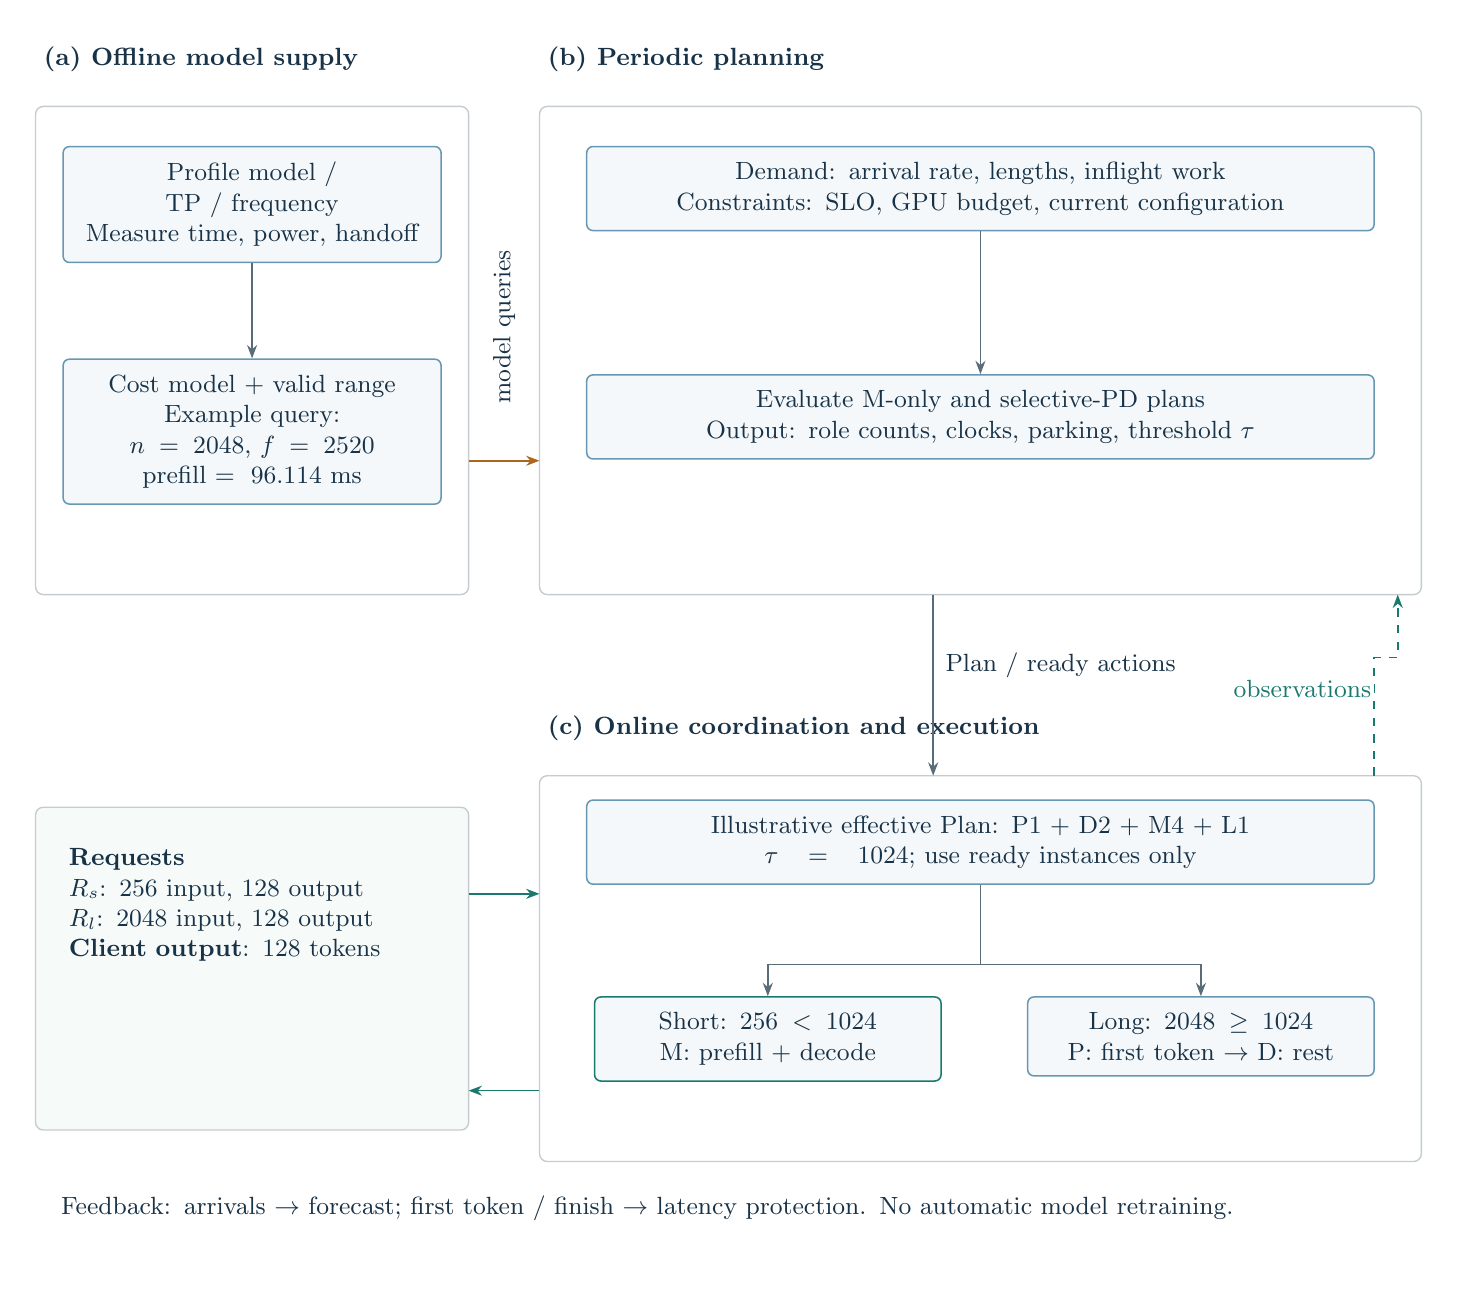
\begin{tikzpicture}[x=1mm,y=-1mm]
\path[use as bounding box] (0,0) rectangle (178,157);
\node[paneltitle] at (2,4) {(a) Offline model supply};
\node[paneltitle] at (66,4) {(b) Periodic planning};
\draw[panel] (1,10) rectangle (56,72);
\draw[panel] (65,10) rectangle (177,72);
\node[box,text width=44mm,anchor=north] (sample) at (28.5,15)
  {Profile model / TP / frequency\\Measure time, power, handoff};
\node[box,text width=44mm,anchor=north] (model) at (28.5,42)
  {Cost model + valid range\\Example query: $n=2048$, $f=2520$\\prefill $=96.114$ ms};
\draw[arr] (sample.south) -- (model.north);
\node[box,text width=96mm,anchor=north] (forecast) at (121,15)
  {Demand: arrival rate, lengths, inflight work\\Constraints: SLO, GPU budget, current configuration};
\node[box,text width=96mm,anchor=north] (plan) at (121,44)
  {Evaluate M-only and selective-PD plans\\Output: role counts, clocks, parking, threshold $\tau$};
\draw[arr] (forecast.south) -- (plan.north);
\draw[arr,draw=orange] (56,55) -- (65,55);
\node[rotate=90,fill=white,inner sep=.2mm,font=\fontsize{9}{11}\selectfont] at (60.5,38) {model queries};
\node[paneltitle] at (66,89) {(c) Online coordination and execution};
\draw[panel] (65,95) rectangle (177,144);
\node[box,text width=96mm,anchor=north] (effective) at (121,98)
 {Illustrative effective Plan: P1 + D2 + M4 + L1\\$\tau=1024$; use ready instances only};
\node[box,text width=40mm,anchor=north,draw=teal] (mixed) at (94,123)
 {Short: $256<1024$\\M: prefill + decode};
\node[box,text width=40mm,anchor=north] (pd) at (149,123)
 {Long: $2048\ge1024$\\P: first token $\to$ D: rest};
\draw[arr] (effective.south) -- (121,119) -| (mixed.north);
\draw[arr] (121,119) -| (pd.north);
\draw[arr] (115,72) -- (115,95);
\node[anchor=west,fill=white,inner sep=.5mm] at (116,81) {Plan / ready actions};
\draw[arr,dashed,draw=teal] (171,95) -- (171,80) -- (174,80) -- (174,72);
\node[anchor=east,fill=white,inner sep=.3mm,text=teal] at (171,84) {observations};
\draw[panel,fill=teal!4] (1,99) rectangle (56,140);
\node[align=left,anchor=north west,text width=48mm] at (4,103)
 {\textbf{Requests}\\$R_s$: 256 input, 128 output\\$R_l$: 2048 input, 128 output\\\textbf{Client output}: 128 tokens};
\draw[arr,draw=teal] (56,110) -- (65,110);
\draw[arr,draw=teal] (65,135) -- (56,135);
\node[anchor=west,align=left,text width=172mm] at (3,150)
 {Feedback: arrivals $\to$ forecast; first token / finish $\to$ latency protection. No automatic model retraining.};
\end{tikzpicture}
\end{document}
